\clearpage
\section{UI Prototype Evolution: PA1 to PA2}
\label{sec:ui-prototype-evolution}

\noindent\textbf{Summary of UI Changes}

\begin{tabularx}{\textwidth}{|L{3.4cm}|Y|}
\hline
\textbf{Area} & \textbf{PA2 update}\\ \hline
Navigation & \textcolor{instructionblue}{A top menu provides access to each role's functions on desktop and mobile.}\\ \hline
Role workspaces & \textcolor{instructionblue}{Separate workspaces for patients, HCPs, medical reviewers, administrators and technical support.}\\ \hline
Patient dashboard & \textcolor{instructionblue}{Medication counts, active reminders and pending review requests appear together, with direct access to health summaries.}\\ \hline
Patient-HCP communication & \textcolor{instructionblue}{Patients can reply within a case; follow-up questions return the case to the HCP review queue.}\\ \hline
Medication reminders & \textcolor{instructionblue}{Pending schedules show their confirmation status, alongside dose recording and adherence history.}\\ \hline
Chatbot access & \textcolor{instructionblue}{The floating chatbot shortcut is retained for quick access from patient screens.}\\ \hline
Health summaries & \textcolor{instructionblue}{Patients can preview, save and share a selected summary with an HCP after giving consent.}\\ \hline
Medication-data review & \textcolor{instructionblue}{A dedicated reviewer screen presents records, supporting evidence and review decisions.}\\ \hline
Administration & \textcolor{instructionblue}{Account and role management is accompanied by a separate activity-history screen.}\\ \hline
Technical support & \textcolor{instructionblue}{Users can report issues; support staff can track requests, add progress notes and update their status.}\\ \hline
\end{tabularx}

\smallskip
{\small Black text describes the PA1 baseline; \textcolor{instructionblue}{blue text highlights PA2 updates}.}

\begingroup
\raggedright
\captionsetup{hypcap=false}
\newcommand{\PAOneImage}[2]{%
  \medskip
  \noindent\begin{minipage}{\linewidth}
    \centering
    \includegraphics[width=\linewidth,height=0.72\textheight,keepaspectratio]{sections/pa1-original/#1.png}
    \captionof{figure}{PA1 reference: #2. Original PA1 screenshot supplied by the project author.}
  \end{minipage}\par
}
\newcommand{\UIRevisionFigure}[6][]{%
  \clearpage
  \subsection{#2}
  \noindent\textcolor{instructionblue}{\textbf{#3}}\par
  \noindent\textbf{PA1 baseline.} #5\par
  \def\OldScreen{#1}%
  \ifx\OldScreen\empty
    \noindent\textit{No directly corresponding screenshot is present in the supplied PA1 set; the PA2 interface is shown below.}\par
  \else
    \PAOneImage{#1}{#2 - baseline or related context}
    \def\IntakeScreen{intake}%
    \ifx\OldScreen\IntakeScreen
      \clearpage
      \noindent\textbf{Medication Entry and Confirmation - PA1 verification step}\par
      \noindent The separate verification screen below completes the PA1 input workflow.\par
      \PAOneImage{verify}{Medication verification}
    \fi
    \clearpage
    \noindent\textbf{#2 - PA2}\par
  \fi
  \noindent\textcolor{instructionblue}{\textbf{PA2 change.} #6}\par
  \medskip
  \noindent\begin{minipage}{\linewidth}
    \centering
    \includegraphics[width=\linewidth,height=0.69\textheight,keepaspectratio]{sections/ui-images/#4}
    \captionof{figure}{PA2 prototype: #2. Fictional demonstration data.}
  \end{minipage}\par
}

\UIRevisionFigure[login]{Role-based Sign-in}{Updated screen | UC-01}{login.png}{PA1 provided patient sign-in and a separate HCP sign-in screen; the administration overview listed patient, HCP and administrator demo roles.}{PA2 provides five demonstration roles: patient, HCP, dataset reviewer, administrator and technical support. Each role opens its own workspace. Incorrect credentials, blocked accounts and unavailable permissions can be demonstrated without granting a session.}

\UIRevisionFigure[dashboard]{Patient Workspace}{Updated screen | UC-02-UC-13}{patient-home.png}{PA1 already showed the next dose, a medication cabinet, dose-recording progress, upload actions and caregiver/profile access.}{PA2 reorganizes these tasks into a top menu and adds visible counts for active reminders and pending review requests, plus direct health-summary access and a floating chatbot shortcut. Daily medication tracking itself is inherited from PA1.}

\clearpage
\noindent\textbf{Top Menu and Chatbot Shortcut - PA2}\par
\textcolor{instructionblue}{The Menu button opens the available functions below the header for each role. Choosing a function closes the menu. Patients can select ``Hỏi Tiểu Bạch'' to open the medication assistant directly.}\par
\medskip
\noindent\begin{minipage}{\linewidth}
\centering
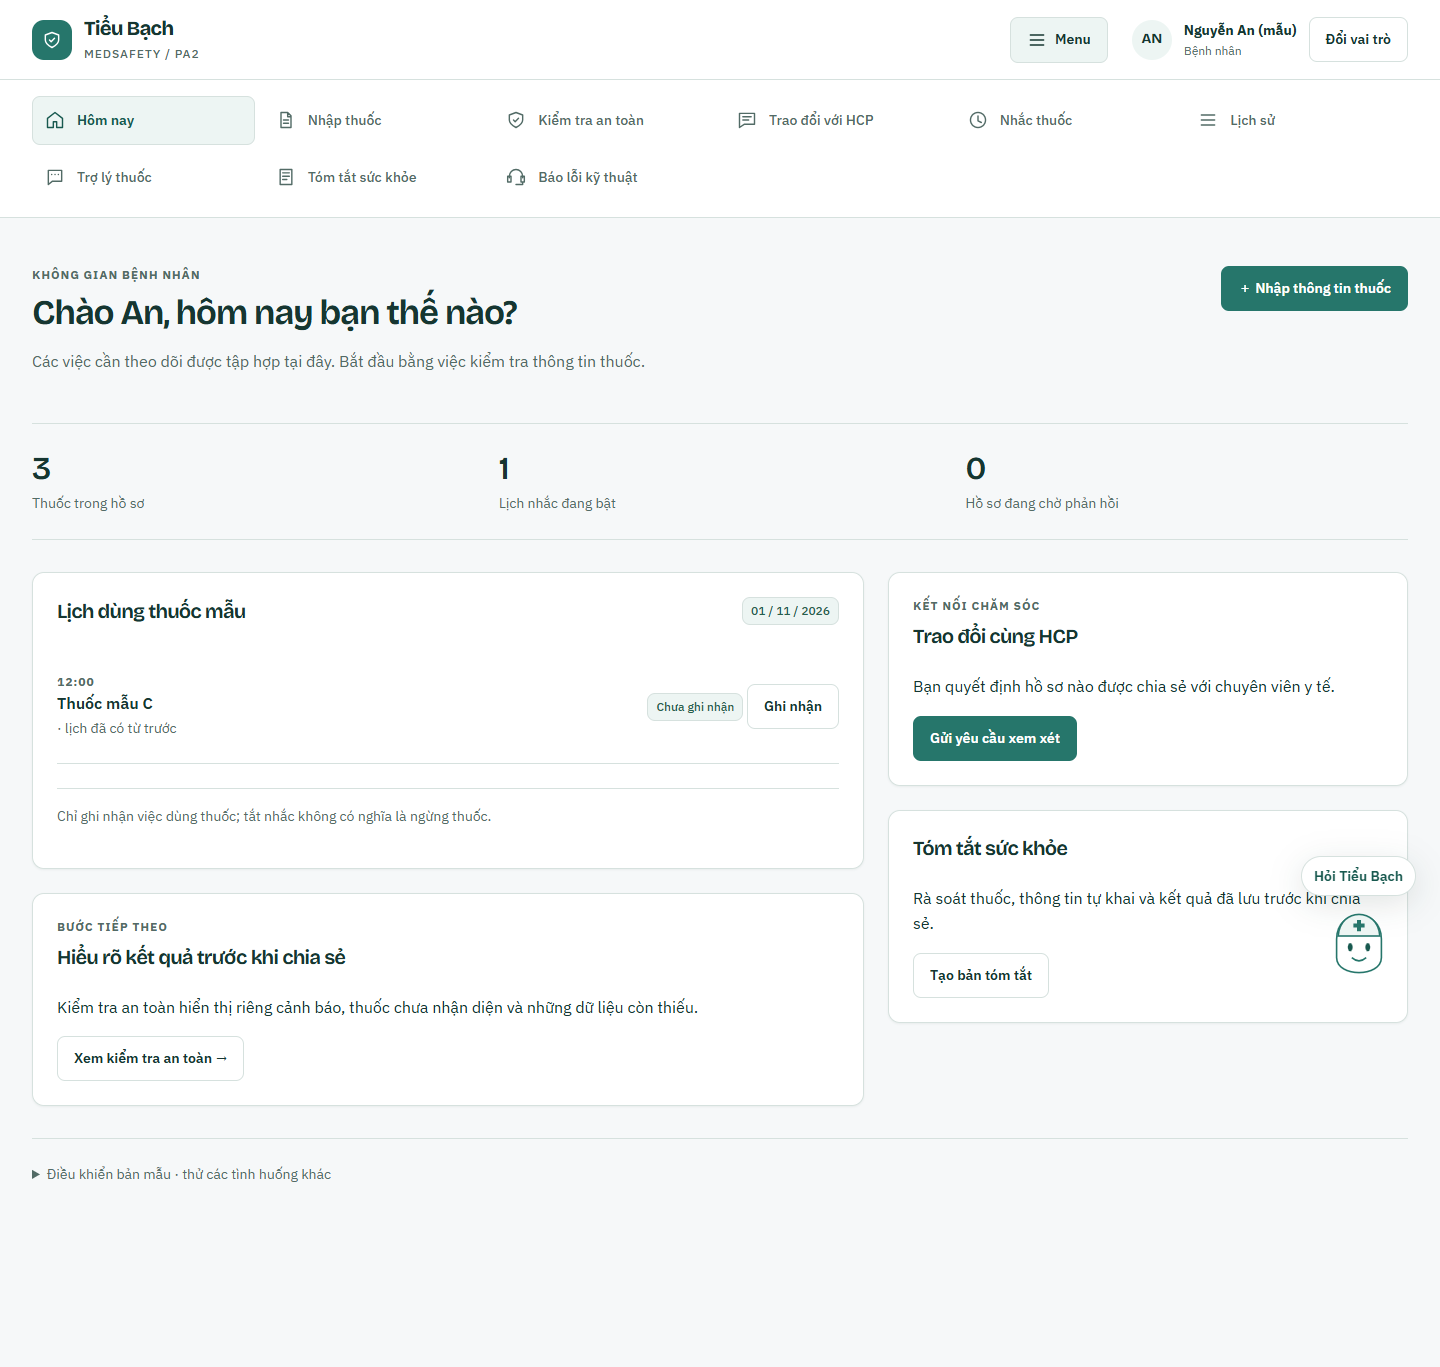
\includegraphics[width=\linewidth,height=0.72\textheight,keepaspectratio]{sections/ui-images/patient-menu.png}
\captionof{figure}{PA2 top menu and patient chatbot shortcut.}
\end{minipage}


\UIRevisionFigure[intake]{Medication Entry and Confirmation}{Updated screen | UC-02}{patient-intake.png}{PA1 separated medication intake and source verification into two pages.}{PA2 combines editable medication rows and explicit patient confirmation in one workflow. Unknown ingredients or strengths remain incomplete rather than being inferred. Image and voice inputs load fictional examples; they do not perform real OCR or speech recognition.}

\UIRevisionFigure[results]{Safety Assessment}{Updated screen | UC-03}{patient-safety.png}{PA1 showed an interaction example, source-coverage limitations, a professional review request and a new-reminder hold pending HCP confirmation.}{PA2 explicitly separates interaction and duplicate-ingredient checks, stores assessment revisions and exposes incomplete-check scenarios. The safety restriction on new reminders and preservation of existing reminders refine behaviour already represented in PA1.}

\UIRevisionFigure[hcp-review]{Patient-HCP Case Conversation}{Extended workflow | UC-04-UC-05}{patient-review.png}{PA1 already allowed a patient to enter a question, view included medications and consent to creating an HCP review request.}{PA2 extends the request into a chronological case conversation with reply-to quotations. Follow-up questions return the same case to Pending HCP Response. Consent is retained from the PA1 request flow rather than introduced for the first time.}

\UIRevisionFigure[hcp-queue]{HCP Review Queue}{Updated screen | UC-05}{hcp-queue.png}{PA1 already had a case-review queue with status counts, a search field, priority selection, patient identifiers and assessment actions.}{PA2 emphasizes patient follow-up status and a new-reply indicator, with each item opening its linked conversation. The PA2 list is simpler: PA1 priority sorting, search and CSV export are not implemented in this version.}

\UIRevisionFigure[hcp-confirmation]{HCP Review and Schedule Confirmation}{Extended workflow | UC-05}{hcp-review.png}{PA1 already provided medication verification, assessment and a confirmation/reply step, including a checkbox for simulated schedule confirmation.}{PA2 places replies, findings and pending schedules in one workspace. It adds reply-to context and explicit Awaiting Patient Response / Pending HCP Response transitions. Schedule confirmation continues an existing PA1 concept; only an eligible recorded confirmation releases relevant pending reminders.}

\UIRevisionFigure[reminders]{Medication Reminders and Dose Recording}{Updated screen | UC-06-UC-08}{patient-reminders.png}{PA1 already showed a day selector, scheduled doses, Taken/Skip actions, undo recording, reminder toggles and a notice requiring professional confirmation for timing changes.}{PA2 separates Taken, Missed and Skipped, records corrections, and displays pending timing proposals without replacing the current schedule. Reminder gating is retained and made explicit; it is not a wholly new PA2 capability.}

\UIRevisionFigure[medications]{Medication and Assessment History}{Expanded history view | UC-09-UC-10}{patient-history.png}{PA1 included a searchable My Medications screen with confirmation-status filters. Its dashboard also linked to medication-use history; the supplied set does not show a separate historical assessment page.}{PA2 adds a combined dose-history and saved-assessment view with medicine, date and status filters. Saved assessments retain their medication revision and are labeled when outdated.}

\UIRevisionFigure[chatbot]{Medication Chat Assistant}{Updated screen | UC-11}{patient-chat.png}{PA1 offered sample explanations of results and questions to discuss with a professional.}{PA2 adds a context-permission control, clarification and information-limit responses, and links to separate confirmation workflows. Requests to modify records do not change data directly. Responses remain scripted examples, without an AI model or clinical inference.}

\UIRevisionFigure[profile]{Patient Health Summary}{New screen | UC-12-UC-13}{patient-summary.png}{PA1 included personal profile fields but no confirmed summary snapshot and sharing workflow.}{PA2 lets the patient create a draft, correct supported self-reported details and save a confirmed snapshot. Sharing is a separate consent step for a selected recipient. Saving alone does not expose the summary to an HCP; missing and outdated information remains visible.}

\UIRevisionFigure{Shared Summaries for HCP}{New screen | UC-13}{hcp-shared.png}{PA1 did not provide an HCP view of explicitly shared summary snapshots.}{PA2 displays only summaries shared through the patient workflow. Each summary preserves its date and medication snapshot; an outdated version is identified. Sharing a case and sharing a summary are separate permissions in the prototype flow.}

\UIRevisionFigure[hcp-database]{Medication Dataset Review}{New reviewer decision screen | UC-14}{reviewer-dataset.png}{PA1 had an HCP drug-database screen and an administration source overview showing DAV/DDInter connection status and outstanding mapping work; the supplied images do not show per-record reviewer decisions.}{PA2 assigns dataset decisions to a dedicated reviewer workspace. It displays the candidate mapping, source evidence, version and decision history. Accept is disabled for missing evidence or an inconsistent mapping; Reject and Needs Correction require a reason. A decision does not automatically publish data or certify clinical validity.}

\UIRevisionFigure[admin]{Account and Role Management}{Expanded administration | UC-15}{admin-accounts.png}{The PA1 administration overview listed three demonstration roles and explicitly stated that account management and server authorization were not implemented.}{PA2 provides editable accounts with multiple roles, account status and confirmation before saving. Duplicate email addresses and removal of the last active administrator are rejected. Administrative access does not automatically reveal patient medical content.}

\UIRevisionFigure[admin]{Administrative Activity History}{New dedicated screen | UC-16}{admin-audit.png}{The PA1 administration page contained a traceability-status panel explaining that an immutable audit log was not implemented.}{PA2 records local account-management actions with actor, time and target. The administrator can filter by account or action text and date. The screen contains administrative metadata rather than patient clinical content.}

\UIRevisionFigure{Report a Technical Issue}{New screen | UC-17}{patient-support.png}{PA1 did not include ticket submission and reporter-visible progress.}{PA2 adds issue category, description and optional minimal diagnostic information. The reporter receives a ticket identifier and can answer a request for further technical details. A private-data scenario blocks submission until the sample attachment is removed.}

\UIRevisionFigure{Technical Support Queue}{New screen | UC-18}{support-tickets.png}{PA1 did not have a dedicated technical-support workspace.}{PA2 shows permitted tickets, technical diagnostics, progress notes and status updates. Support can request more information or record a resolution. Medical content is excluded from the diagnostic fixture; clinical review and dataset acceptance are not support actions.}

\UIRevisionFigure{Mobile Patient Workspace}{PA2 responsive view; PA1 mobile capture unavailable}{mobile-viewport.png}{The supplied PA1 profile image shows text-size and contrast controls, but the set contains no mobile-viewport screenshot. The earlier re-captured mobile image is not used as the official baseline.}{PA2 provides the same top menu on mobile, stacked panels and a floating chatbot shortcut. Dedicated text-size/contrast and caregiver-contact controls shown in PA1 are not implemented in the current PA2 scope. This view must not be read as evidence that PA1 lacked responsive support.}

\endgroup
\clearpage
